


%================================================================= %

\subsection{Nonlinearity}

\begin{framed}

\begin{verbatim}	
	

# Evaluate Nonlinearity

# component + residual plot 


crPlots(fit)


# Ceres plots 

ceresPlots(fit)


\end{verbatim}

\end{framed}

%http://stats.stackexchange.com/questions/58141/interpreting-plot-lm
%\texttt{I explained the assumption of homoscedasticity and the plots that can help you assess it (including scale-location plots [2]) on CV here: What does having constant variance in a linear regression model mean? I have discussed qq-plots [3] on CV here: QQ plot does not match histogram. So, what's left is primarily just understanding [5], the residual-leverage plot.}
In a multiple linear regression, it is assumed that the dependence on each of the predictors is linear. The partial residual plot has been available as a diagnostic, but it can fail if there are nonlinear relationships among the predictors. The Mallows augmented partial residual plot is effective even if there are quadratic relationships among the predictors. Dennis Cook developed the CERES plot to show a curve in the relationship of the dependent variable to a predictor, in spite of any nonlinear relationships among the predictors.
\end{document}

Non-constant Error Variance
# Evaluate homoscedasticity
# non-constant error variance test
ncvTest(FitAll)
# plot studentized residuals vs. FitAllted values 
spreadLevelPlot(FitAll)
spread vs. levels click to view

%%%%%%%%%%%%%%%%%%%%%%%%%%%%%%%%%%%%%%%%%%%



#### Non-constant Error Variance}

```{r}

# Evaluate homoscedasticity
# non-constant error variance test
ncvTest(FitMod)
# plot studentized residuals vs. fitted values 
spreadLevelPlot(FitMod)



```{r}
> ncvTest(FitMod)
Non-constant Variance Score Test 
Variance formula: ~ fitted.values 
Chisquare = 3.330027    Df = 1     p = 0.06802577 


%mtcarsSpreadLevel Plot here

\begin{figure}[h!]
\centering
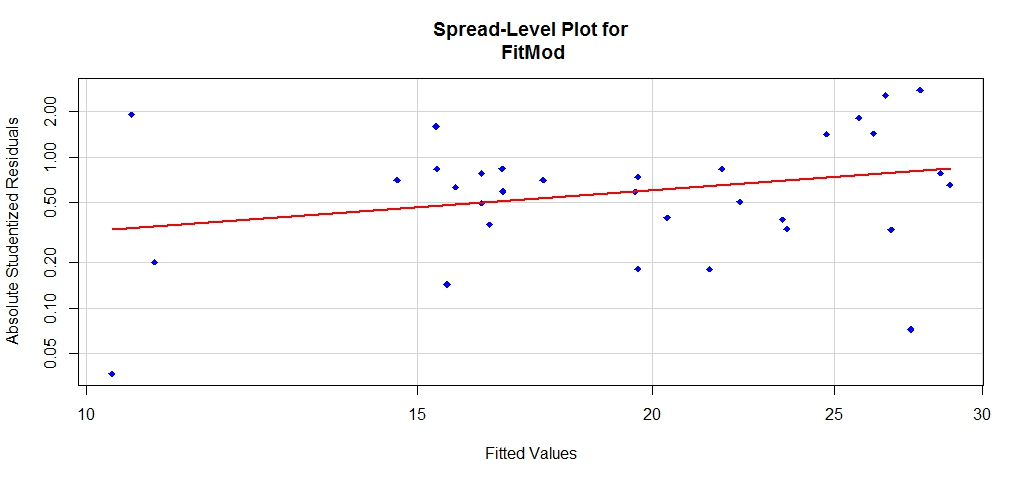
\includegraphics[width=0.7\linewidth]{./mtcarsSpreadLevelPlot}
\label{mtcarsSpreadLevelPlot}
\end{figure}


```{r}
Suggested power transformation:  0.08866484 
